\chapter{Comparing JavaScript Frameworks}
\label{comparing-frameworks}

\todo{leírni miért js!!}

For the project, I preferred to choose a JavaScript framework for faster development than using plain JavaScript with jQuery. Writing every component from scratch needs a lot of time. Hundreds of developers contribute in open-source frameworks, and developers can utilize their reviewed and tested work. This leads to getting more tasks done in less time. Because this project follows the MVC pattern \see{mvc}, only JavaScript MVC frameworks will be compared. The TodoMVC~\cite{TodoMVC} website helps developers to select a JavaScript MVC framework for their project. It provides the same example written in JavaScript using different JavaScript MVC frameworks.

During comparison I checked the followings:
\begin{itemize}
	\item \textbf{AJAX requests:} the client and the server \see{fig:conceptional-system-design} will communicate via REST using JSON format.
	\item \textbf{data binding:} to connect the data from the model to the view \see{fig:classic-mvc-webapplication}.
	\item \textbf{routing:} to build a single-page application.
\end{itemize}

\bence{4. eleje: amiről még beszéltünk, hogy ellenőrizni kéne: különböző tesztelési módszerek alkalmazhatósága,}

In a single-page application (SPA) when the user opens the web site in a browser, all the resources will be downloaded with a single page load. From that point when the user interacts with the web site, it will dynamically update previously downloaded single page~\cite{SPA}.

In JavaScript with \emph{AJAX requests} we can send requests to a server asynchronously without reloading a page. In a SPA we want to make the browser think it is always on the same page. When the user clicks on a new link, the browser will not reload the whole page, it will just simply load the new view into the old frame. Everything happens in the background so the application will not force the user to wait while it sends data to a server. If the application is retrieving data, then when it arrives, the application can process it and show the result to the user.

The classic \emph{data binding} model is when the view template and the data from the model are merged together to create the to be displayed view. Any data changes in the view will not automatically sync into the model. The developer has to write the controller that syncs the changes between the model and the view~\cite{Angular-Developer-DataBinding}.

Upon URL change an SPA will not download a new page. It will navigate to the right part of the application. \emph{Routing} takes care of this automatically. The SPA needs a routing table to know which URL belongs to which controller or view.

During the comparison I made a small test program in every JavaScript framework to try AJAX requests, data binding and routing. The source codes are publicly available on Github with a gulp file \see{gulp} and an API blueprint test file for Drakov \see{api-blueprint}.

\section{React}

My first choice was React~\cite{React}. It is developed by Facebook and Instagram since 2013.

React creates a virtual DOM instead of always updating the browser's actual document object model (DOM)~\cite{dom}. The DOM provides a structured representation of HTML and XML documents. The objects are the nodes of the tree, and the tree structure is the DOM tree. In this case the DOM connects the HTML page to the JavaScript code. The virtual DOM is like a blueprint of the real DOM. Instead of containing a div\footnote{A div is a generic container in HTML. It helps structuring the HTML document~\cite{div}.} element, the virtual DOM contains a React.div element that is just data and not a rendered content. React is able to find out what has changed on the real DOM. It makes changes to the virtual DOM, because that is faster and then re-render the real DOM~\cite{React-Virtual-DOM}.

To create DOM elements, we can choose between JavaScript and JSX~\cite{JSX}. If we use JavaScript, then the code will render the HTML code for us. If we choose JSX, then we can mix JavaScript and HTML-like syntax, and we can insert the desired HTML code as the return statement. 

For data binding React has a one-way data flow called Flux~\cite{Flux}. Flux supports data flow only in a single direction, downstream. This means if something is changed in the component tree, then it will cause the element to re-render itself and all of its descendants.

React focuses only on building views. The core React version does not have an option for routing and AJAX requests. If I want to support those in my application, then React should be combined with other frameworks or libraries to have a full MVC experience.

\newparagraph{Test Program~\cite{Github-react}}
The components are separated into different JavaScript files. JSX was used to represent the views. Before the concatenation a JSX transformer converts the inline HTML-like JSX to JavaScript code. The React components' states were used as a model. Because React has not got an option for AJAX requests, jQuery was used to download some mock data from the mock server. React Router was used~\cite{React-router} for routing. 

\section{AngularJS}

AngularJS~\cite{Angular} is one of the most advanced JavaScript frameworks nowadays.  It has been maintained by Google for 6 years. It focuses mostly on dynamic views in web-applications. 

Creating a website is done with an extended HTML vocabulary, like Android Layouts where we declare everything in XML.  It uses a two-way data binding template~\cite{Angular-Developer-DataBinding} which means whenever either the View or the Model is changed, it will update the other one automatically.

Angular AJAX requests are similar to the AJAX methods in jQuery, but Angular takes care of setting headers and converting the data to JSON string. It can also be used in unit tests with ngMock~\cite{Angular-AJAX}, because it can create a mock server. 

For routing Angular uses a special listener. It binds these listeners to links. If the user clicks on a link, Angular will simply push the page to the browser's history and replace the view with the new page. This will even allow the back button to operate. This method works only if the website is loading from a server, because it allows Angular to load into the memory otherwise the listeners cannot navigate through the pages~\cite{Angular-Location}~\cite{Angular-Location2}.

\newparagraph{Test Program~\cite{Github-angular}}
The controllers are separated into different JavaScript files and the views into different HTML templates. The routing connects the right HTML template to the right controller. The JavaScript files are concatenated using gulp. The HTML templates are in different HTML files. Variables inside the controllers were used as a basic model. The routing is not included in the core Angular framework, but Google provides a library for it.

\section{Mithril}

Mithril~\cite{Mithril} is a small MVC framework created by Leo Horie. It uses a similar virtual DOM like React, but also implements controller features like routing.

When we are creating a website, Mithril first creates virtual DOM elements, that is a JavaScript object that represents a DOM element. Rendering will create a real DOM element from the virtual one~\cite{Mithril-m}~\cite{Mithril-render}. If we prefer using HTML syntax, we can use MSX~\cite{MSX}. It uses JSX, but transforms the output to be compatible with Mithril. 

Mithril has one-way data flow, from the model to the view. It has an auto-redrawing system to ensure that every part of the UI is up-to-date with the data. It uses a diff algorithm to decide which parts of the DOM needs to be updated and nothing else will be changed. Mithril automatically redraws after all controllers are initialized and will diff after an event handler is triggered. It also supports non-Mithril events to trigger auto-redrawing~\cite{Mithril-redraw}. If we need view-to-model direction, Mithril provides us an event handler factory. This returns a method that can be bound to an event listener~\cite{Mithril-withAttr}.


Mithril provides a utility for AJAX requests. We can set an early reference for the asynchronous response and queue up operations to be performed after the request completes.  ~\cite{Mithril-webservice}~\cite{Mithril-request}.


For routing Mithril needs a key-value map of possible routes and Mithril modules to connect the routes to the modules. Upon routing the module's controller will be called and passed as a parameter to the view.~\cite{Mithril-routing}.

\newparagraph{Test Program~\cite{Github-mithril}}
A Mithril module contains a model, a controller and a view. A controller is a JS constructor and the view is a function, that returns a virtual DOM. Modules are separated into different JavaScript files and concatenated with gulp. MSX transformer converts the HTML-like MSX to JavaScript code.

\newpage
\section{Comparison Table}

\begin{center}
	\begin{table}[!htbp]
		\begin{tabular}{|p{3cm}||p{3.5cm}|p{3.5cm}|p{3.5cm}|}\hline
									& \multicolumn{1}{c|}{\textbf{React}}          
									& \multicolumn{1}{c|}{\textbf{Angular}}   
									& \multicolumn{1}{c|}{\textbf{Mithril}} \tabularnewline \hhline{|=#=|=|=|}
		\multicolumn{1}{|c||}{\multirow{7}{*}{\textbf{AJAX requests}}}      
									& Not part of the core framework. Requires an external library or framework.          
									& Provides simple AJAX methods. It can be used for unit tests, because it can create a mock server.
									& Provides a simple utility. An early reference can be set for the response to qeue up operations to be performed after the request completes. \tabularnewline\hline
		\multicolumn{1}{|c||}{\multirow{7}{*}{\textbf{data binding}}} 		
									& One-way data flow, downstream. if something is changed in the component tree, it re-renders itself and all of its descendants.
									& Two-way data binding. Either the model or the View is changed, it will update the other one autimatically.    
									& One-way data flow. Uses a diff algorithm, that decides which part of the DOM needs to be updated. It is triggered by event handlers.   \tabularnewline\hline
		\multicolumn{1}{|c||}{\multirow{6}{*}{\textbf{routing}}}        	
									& Not part of the core framework. Requires an external library or framework.         
									& A special listener is binded to the links. It pushes the page to the browser's history.
									& Uses a key-value map as a routing table, that connects the URLs with Mithril module controllers.    \tabularnewline \hline
	\end{tabular}
	\caption{Framework Comparison Table}
	\label{table:frameworkcomparison}
	\end{table}
\end{center}


\section{Conclusion}
In performance both React and Mithril are faster than Angular, because they use virtual DOM. Angular's public API interface is much bigger than React's or Mithril's. React does not have routing and AJAX requests in its core library, so it depends on other libraries. 
I choose Mithril for this project, because it is  self-contained, so it does not have to depend on other libraries. It has utilities built-in for routing and AJAX requests. And it has a small API with great documentation. 

\section{Supported Web Browsers}
At first I am aiming to develop the portal for desktop browsers. The portal will support every browser, that is supported by Google~\cite{google-support}.
The supported browsers are:
\begin{itemize}
	\item Chrome
	\item Internet Explorer
	\item Firefox
	\item Safari
\end{itemize}

\subsection{Internet Explorer}
The portal will support Internet Explorer 10 and every newer version~\cite{google-support-blog}.

Because there are some features, that Mithril depends on and are not part of earlier Internet Explorer version, I added a shim JavaScript file to the project~\cite{Mithril-tools}. 

To force Internet Explorer to render in the highest available mode, I added a special meta tag in the html file~\cite{IE10-microsoft}~\cite{IE10-html5-boiler} \see{html-impl}.

\section{Frontend System Design}
\label{frontend-system-design}
The front end system design depends on the chosen framework's behavior and it also depends on which software architecture pattern is used. This project follows the MVC pattern. In this section I am going to introduce the general MVC pattern and the final front end system design. 

\todo{Marshalling helyett talán jobb a "serialization" -> ábrán kijavítani}

\section{MVC Pattern}
\label{mvc}

The Model-View-Controller (MVC) is a software architecture pattern for user interface implementation, where the application logic is separated from the user interface.

In object-oriented programming the Model is the objects where the data from the database is stored. The View is the presentation layer. The user sees and interacts with the View. The Controller will process and respond to the user requests and invoke the changes in the Model. 

%The MVC pattern is memory efficient, because multiple views can share the same underlying data model. Controllers can be separated by events. This allows the developer to create a controller hierarchy, because a controller for a keyboard event is different from a controller for a mouse event. Views implement an instance of a controller, that can be changed at run-time, because we can be disabled and enabled.

%\bence{Az az érzésem, hogy ezt valahonnan másoltad / fordítottad.  Ha igen, illik hivatkozást betenni a szöveg végére.  Ha nem, akkor erről beszéljünk, mert a memória-hatékonyság ebben a formában szerintem nem igaz az MVC-re.  Nem lesz valami hatékony azért, mert MVC minta alapján készül.}

\subsection{MVC Web Applications}
\todo{Marshalling helyett talán jobb a "serialization" -> ábrán kijavítani}

\begin{figure}[!ht]
	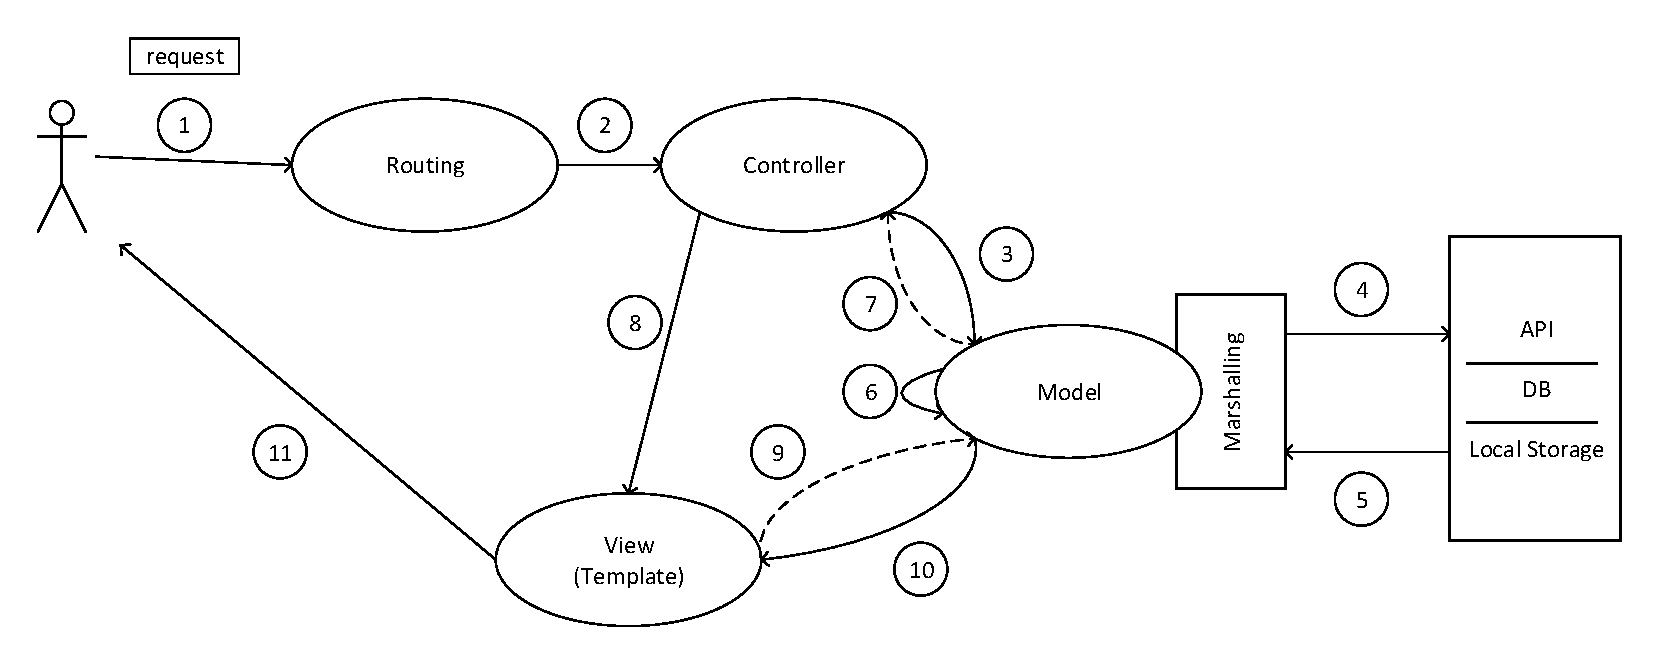
\includegraphics[width=\textwidth]{figures/klasszikus_mvc_webalkalmazas.pdf}
	\caption[Classic MVC Web Application]{Classic MVC Web Application~\cite{mvc-webapp}}
	\label{fig:classic-mvc-webapplication}
\end{figure}

In web applications the browser communicates with a controller. When the user sends a request, routing will decide which controller will handle the request. The chosen controller talks to the model to get the relevant data. If it is necessary, the model will send data to or ask for data from the database, the API or the local storage. During this process, the data has to be transformed via serialization. serialization is the process, that transforms the data between storable and sendable dataformats. When the model returns the desired data to the controller, it will forward the data to the view. The presentation layer will decide which page has to be returned to the browser, binds the data to the view template and returns it.

\subsection{Final Front End System Design}

The final design is based on the classic MVC Web application \see{fig:classic-mvc-webapplication} and the behavior of Mithril~\cite{Mithril-getting-started}. It describes the design of the client, but does not describe how the clients communicate with each other, because the different clients cannot communicate with each other.

The routing component handles the incoming requests. It uses a routing table to decide which controller has to handle the request.

The controller talks to the model, if any data should be changed or needed. The model sends data to the API or asks for data from the API. Every data is converted between the representation suitable for the implementation and the AJAX requests by the serialization component. The communication between the API and the client is handled by the server communication component.

The controller provides helper methods (e.g. getting data from the model) and it is passed as the first parameter to the view~\cite{Mithril-routing}. The rendered view is forwarded to the browser, that visualized it for the user.

\newpage
\begin{landscape}
	\begin{figure}[!htbp]
		\centering
		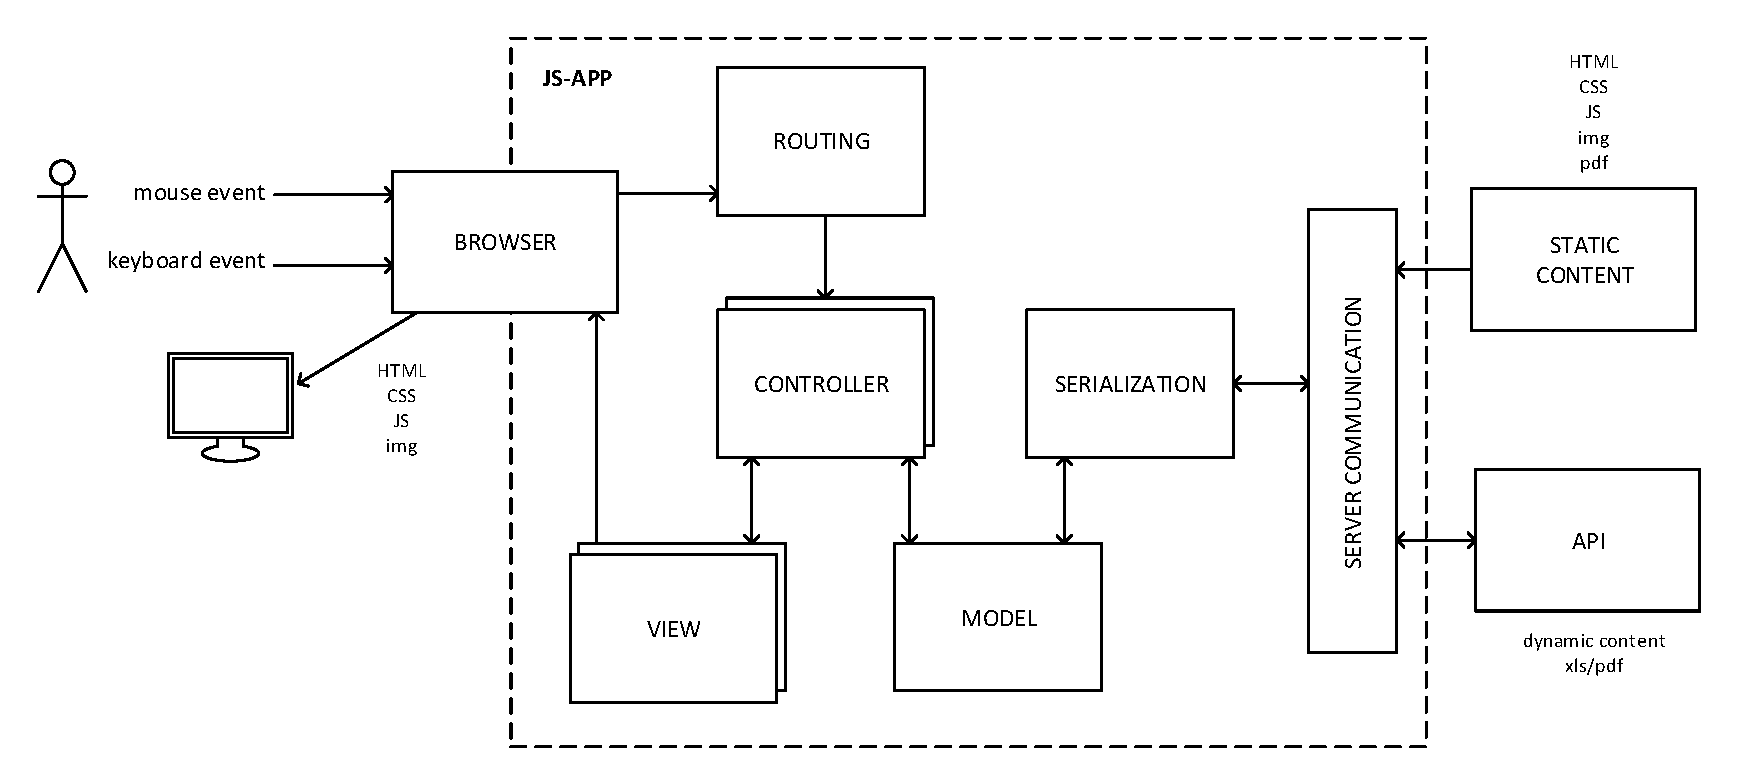
\includegraphics[height=0.8\textwidth]{figures/frontend_rendszerterv.pdf}
		\caption[Front End System Design]{Front End System Design\\The JS-APP was made by me and the outer layer was made by Bence Golda.}
		\label{fig:frontend-system-design}
	\end{figure}
\end{landscape}
